% !TEX program = xelatex
\documentclass[11pt]{article}
\usepackage[margin=1in]{geometry}
\usepackage{nopageno} % no page numbers
\usepackage{setspace} % \doublespacing

\usepackage{graphicx}
\graphicspath{ {./graphics/} }
\usepackage[dvipsnames]{xcolor}
\definecolor{CrispBlue}{HTML}{0176AE}

\usepackage{fontspec}
\usepackage{tcolorbox}
\usepackage{etoolbox}
\BeforeBeginEnvironment{verbatim*}{\begin{tcolorbox}[colback=CrispBlue!5!white,colframe=CrispBlue!75!black]}%
\AfterEndEnvironment{verbatim*}{\end{tcolorbox}}%

\usepackage{hyperref}
\hypersetup{
    colorlinks,
    citecolor=black,
    filecolor=black,
    linkcolor=black,
    urlcolor=black
}

\renewcommand{\footnotesize}{\fontsize{8pt}{10pt}\selectfont}

% \usepackage[labelfont={small,sc,bf},textfont={small,sc,bf}]{caption}
\setlength{\parindent}{0pt}
% \setlength{\parskip}{1em}

\usepackage{tocloft}
\renewcommand{\cftpartleader}{\cftdotfill{\cftdotsep}}
\renewcommand{\cftsecleader}{\cftdotfill{\cftdotsep}}

\usepackage[shortlabels]{enumitem}

\usepackage{lastpage}
\usepackage{fancyhdr}
\pagestyle{fancy}
\fancyhf{}
\renewcommand{\headrulewidth}{0pt}
\rfoot{Page \thepage\ of \pageref*{LastPage}}

\usepackage{amsmath,amsfonts,amssymb}
\usepackage{bm}
\usepackage{mathtools}

\renewcommand{\listfigurename}{List of Figures}

\begin{document}
% \setmainfont{SF Pro Text}
% \setsansfont{SF Pro Text}
% \setmonofont{SF Mono}
% \renewcommand{\familydefault}{\sfdefault}

\hypersetup{
    linkcolor=CrispBlue,
    urlcolor=CrispBlue,
    breaklinks=true
}

David Kirby\\
ECE 520: VLSI Design\\
Spring 2022

\begin{center}
    \large\bfseries Homework \#1
\end{center}

\begin{enumerate}
    \item In order to estimate the fabrication cost, we need to determine the number of dies in a wafer. Prove the equations in slide 61 of Lecture 1. Then, use the equations in the slide to determine the percentage of wasted silicon (due to the edge of the wafer), as a function of die size. Plot the \% wasted area as a function of die size for die sizes from 1 cm to 5 cm in an 8 inch wafer.
    \begin{align}
        \text{yield} &= \frac{\text{\# good chips per wafer}}{\text{total \# of chips per wafer}}\\[1em]
        \text{die cost} &= \frac{\text{wafer cost}}{\frac{\text{dies}}{\text{wafer}}\times\text{die yield}}\\[1em]
        \frac{\text{dies}}{\text{wafer}} &= \frac{\pi\left(\frac{\text{wafer diameter}}{2}\right)^2}{\text{die area}} - \frac{\pi \times \text{wafer diameter}}{\sqrt{2 \times \text{die area}}}\\[1em]
        \text{wasted area} &= (1 - \text{yield}) \times 100\%
    \end{align}
    \begin{figure}[!ht]
    \centering
    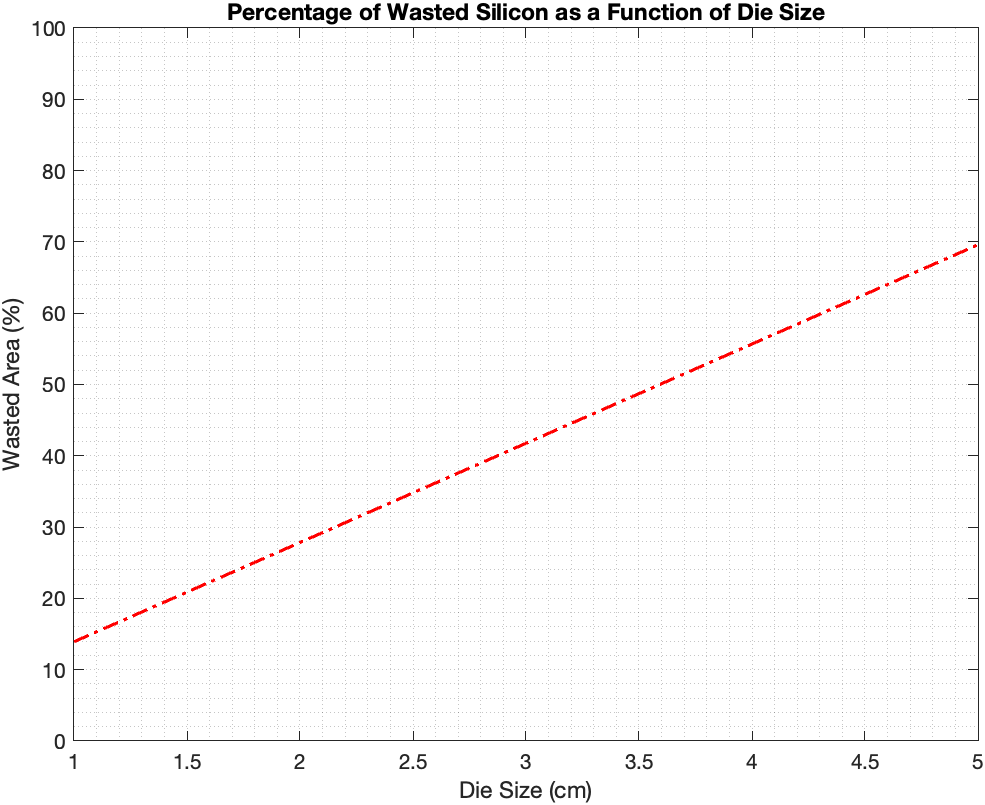
\includegraphics[width=0.65\textwidth]{figure01.png}
    \caption{Percentage of Wasted Silicon as a Function of Die Size}
    \label{fig:figure01}
    \end{figure}

    \item In this problem, we would like to derive the equation for drain current in saturation region considering channel-length modulation. Assume that the change in channel length is proportional to VDS (i.e. \(\Delta L / L = \lambda V_{DS}\)). Show how equation (3.29) in your textbook becomes (3.30) when you include channel length modulation.\vspace{1.5em}
    
    Channel length modulation gives: \( L = L - \Delta L\)
    \begin{align*}
        I_D &= \frac{K'n}{2} \left(\frac{W}{L-\Delta L}\right)\left(V_{gs}-V_t\right)^2\\[1em]
        &= \frac{K'n}{2}\left[ \frac{W}{L}\left(1+\frac{\Delta L}{L}\right)\right]\left(V_{gs}-V_t\right)^2\\[1em]
        &= \frac{K'n}{2}\left[ \frac{W}{L}\left(1+\lambda V_{DS}\right)\right]\left(V_{gs}-V_t\right)^2\\[1em]
        &= I'_D \left(1+\lambda V_{DS}\right)
    \end{align*}
    \item Based on the list of previous VLSI projects for ECE520/424 that we discussed in Lecture 1, please suggest at least one new project that you will be interested to design and work on this semester. Please explain in one paragraph the detail of your suggested project. Feel free to use online resources, if you need to.\vspace{1.5em}
    
    I missed the first few lectures, so I do not know the specifics of the project yet, but in my Advanced Computer Architecture class we discussed a hardware-software codesign using ASICs. I am interested in exploring those more and possibly attempting to design one.
\end{enumerate}

% \begin{figure}[!ht]
%     \centering
%     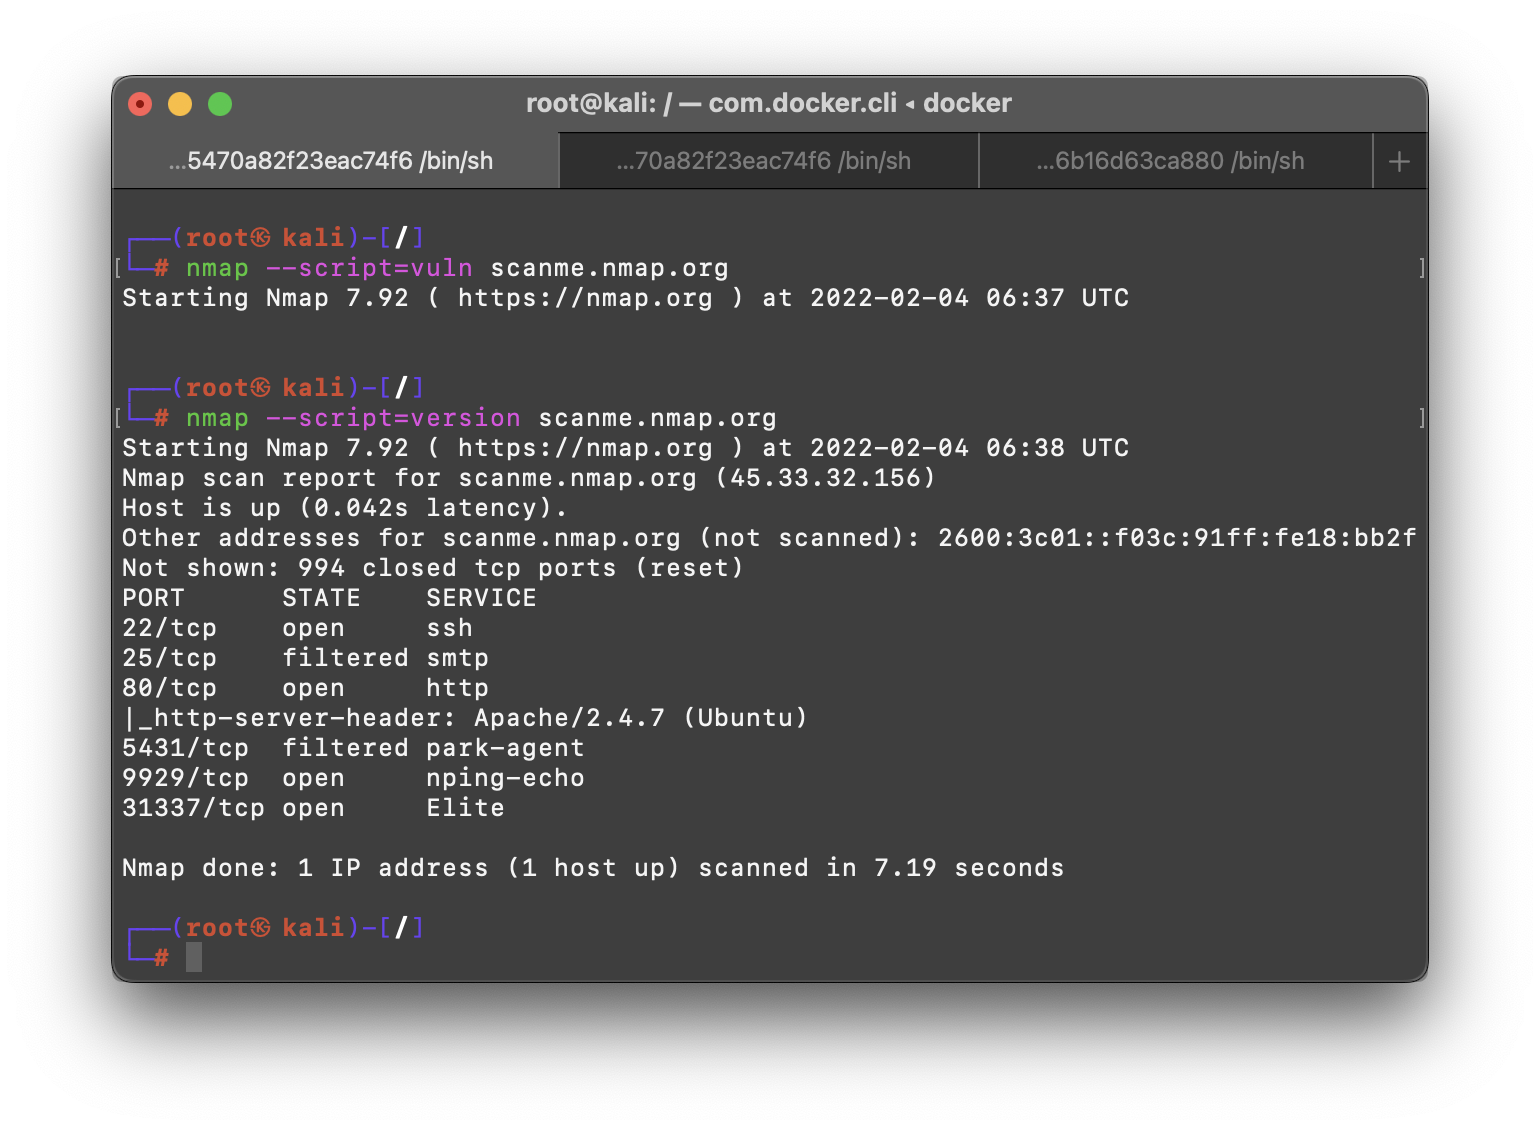
\includegraphics[width=0.8\textwidth]{figure10.png}\vspace{-1em}
%     \caption{Command line for nmap with scripts of scanme.nmap.org.}
%     \label{fig:nmap06}
% \end{figure}


\end{document}